\chapter{Reactiemechanismen: elementaire stappen en benaderingen}\label{ch:b1:elementary-steps}

Stikstofmonoxide, dat in automotoren en bij bliksem ontstaat, verbindt
zich met de zuurstof van de lucht: \ce{2NO + O2 -> 2NO2}. In het
laboratorium gemeten is de snelheid van deze reactie evenredig met
$[\ce{NO}]^2[\ce{O2}]$ --- en ze verloopt \emph{trager} wanneer het gas
verwarmd wordt. Eén enkele botsing van drie moleculen zou het eerste feit
kunnen verklaren, nooit het tweede: elke botsing wordt energierijker met
de temperatuur. De verklaring is dat de reactie geen enkele gebeurtenis
is, maar een opeenvolging van eenvoudiger gebeurtenissen: haar
mechanisme. Dit hoofdstuk definieert die \omterm{def:b1:elementary-steps:elementary-step}{elementaire stappen}, het
\omterm{def:b1:elementary-steps:energy-profile}{energieprofiel} waarlangs ze verlopen, en de benaderingen die van een
mechanisme een \omterm{def:b1:rate-laws:order}{snelheidswet} maken; het eindigt met de katalyse, de kunst
om een gemakkelijker pad te openen.

\begin{recall}
Boek 1 (jaar 12) beschreef een \omterm{def:b1:elementary-steps:elementary-step}{reactiemechanisme} als een opeenvolging van
stappen, getekend met gebogen pijlen, met intermediairen die gevormd en
verbruikt worden, en een \omterm{def:b1:elementary-steps:catalyst}{katalysator} als een deeltje dat een reactie
versnelt zonder verbruikt te worden. \omterm{def:b1:rate-laws:order}{Snelheidswetten}, ordes en de \omterm{thm:b1:rate-laws:arrhenius}{wet van
Arrhenius} werden gedefinieerd in \cref{ch:b1:rate-laws}.
\end{recall}

\section{Elementaire stappen}

\begin{definition}[Elementaire stap, moleculariteit, mechanisme]\label{def:b1:elementary-steps:elementary-step}
Een \emph{elementaire stap}\index{elementaire stap} is een reactie die in
één enkele moleculaire gebeurtenis plaatsvindt, zoals ze geschreven is,
zonder enig intermediair. Haar \emph{moleculariteit}\index{moleculariteit}
is het aantal deeltjes dat in die gebeurtenis reageert: 1
(unimoleculair, een ontleding of omlegging), 2 (bimoleculair, een
botsing), zelden 3. Een
\emph{reactiemechanisme}\index{reactiemechanisme} is de verzameling
elementaire stappen waarvan de som de totale reactie is. Een deeltje dat
in een stap gevormd en in een latere stap verbruikt wordt, en dat in de
totale reactievergelijking ontbreekt, is een
\emph{reactie-intermediair}\index{reactie-intermediair}.
\end{definition}

\begin{proposition}[Snelheidswet van een elementaire stap]\label{prop:b1:elementary-steps:elementary-law}
Een \omterm{def:b1:elementary-steps:elementary-step}{elementaire stap} heeft een orde, en zijn \omterm{def:b1:rate-laws:order}{partiële ordes} zijn gelijk
aan zijn stoichiometrische coëfficiënten: $\mathrm{A} \to \dots$ heeft
$v = k[\mathrm{A}]$;
$\mathrm{A} + \mathrm{B} \to \dots$ heeft $v = k[\mathrm{A}][\mathrm{B}]$;
$2\,\mathrm{A} \to \dots$ heeft $v = k[\mathrm{A}]^2$. Het omgekeerde is
onjuist: een reactie waarvan de ordes gelijk zijn aan de coëfficiënten,
hoeft niet elementair te zijn.
\end{proposition}

\begin{proof}[Redenering]
Een bimoleculaire stap vindt plaats wanneer een \ce{A} een \ce{B}
ontmoet; het aantal van zulke ontmoetingen per volume- en tijdseenheid is
evenredig met het aantal \ce{A} per volume-eenheid en met het aantal
\ce{B}, dus met
$[\ce{A}][\ce{B}]$. Een unimoleculaire stap overkomt elk molecuul met een
vaste kans per tijdseenheid, wat een snelheid evenredig met $[\ce{A}]$
geeft.
\end{proof}

\begin{remark}[Waarom de moleculariteit zelden groter is dan twee]\label{rem:b1:elementary-steps:termolecular}
Dat drie deeltjes elkaar op hetzelfde ogenblik ontmoeten, elk met de
juiste energie en oriëntatie, is een zeldzame gebeurtenis; een reactie
met \omterm{def:b1:rate-laws:order}{totale orde} 3 is bijna altijd het resultaat van twee opeenvolgende
bimoleculaire stappen, zoals in het weekendprobleem.
\end{remark}

\section{Energieprofielen}

\begin{definition}[Reactiecoördinaat, energieprofiel, overgangstoestand]\label{def:b1:elementary-steps:energy-profile}
Tijdens een \omterm{def:b1:elementary-steps:elementary-step}{elementaire stap} bewegen de atomen van de schikking van de
beginstoffen naar die van de reactieproducten; een grootheid die deze
voortgang meet (een bindingslengte die groeit, een andere die krimpt), is
de \emph{reactiecoördinaat}\index{reactiecoordinaat@reactiecoördinaat}.
De grafiek van de potentiële energie van het systeem daarlangs is het
\emph{energieprofiel}\index{energieprofiel}. Het maximum ervan is de
\emph{overgangstoestand}\index{overgangstoestand}, een schikking van de
atomen met half gevormde en half verbroken bindingen, die niet langer
duurt dan een moleculaire trilling en niet geïsoleerd kan worden. De
hoogte van dit maximum boven de beginstoffen is de energiebarrière van de
stap.
\end{definition}

\begin{omfigure}
\begin{tikzpicture}
\begin{axis}[omprofile, name=a,
  width=0.48\linewidth, height=5.4cm, xmin=0, xmax=10, ymin=-68, ymax=95,
  xlabel={reactiecoördinaat}, ylabel={energie}]
\addplot[omDef, very thick] table[x=x, y=E] {figdata/out/bachelor-1-energy-profiles-one-step.dat};
\draw[dashed, black!40] (axis cs:0,0) -- (axis cs:10,0);
\draw[<->, omThm] (axis cs:5,0) -- (axis cs:5,79);
\node[omThm, anchor=west, font=\small] at (axis cs:5.1,30) {barrière};
\draw[<->, omProp] (axis cs:9.9,0) -- (axis cs:9.9,-40);
\node[omProp, anchor=east, font=\small] at (axis cs:9.8,-14) {$\Delta E$};
\node[anchor=south, font=\small] at (axis cs:5,81) {overgangstoestand};
\node[anchor=north west, font=\small] at (axis cs:0.15,-3) {beginstoffen};
\node[anchor=north, font=\small] at (axis cs:8.6,-42) {producten};
\end{axis}
\begin{axis}[omprofile, at={(a.east)}, anchor=west, xshift=1.2cm,
  width=0.48\linewidth, height=5.4cm, xmin=0, xmax=10, ymin=-64, ymax=95,
  xlabel={reactiecoördinaat}, ylabel={energie}]
\addplot[omDef, very thick] table[x=x, y=E] {figdata/out/bachelor-1-energy-profiles-two-step.dat};
\node[anchor=south, font=\small] at (axis cs:3,71) {OT 1};
\node[anchor=south, font=\small] at (axis cs:7,56) {OT 2};
\node[anchor=north, font=\small, align=center] at (axis cs:5,27) {inter-\\mediair};
\node[anchor=north west, font=\small] at (axis cs:0.15,-3) {beginstoffen};
\node[anchor=north east, font=\small] at (axis cs:10,-43) {producten};
\end{axis}
\end{tikzpicture}

{\small Links: het profiel van één \omterm{def:b1:elementary-steps:elementary-step}{elementaire stap}, met zijn barrière en
de energieverandering van de reactie. Rechts: een mechanisme in twee
stappen; het intermediair ligt in een dal tussen twee
\omterm{def:b1:elementary-steps:energy-profile}{overgangstoestanden} (OT). De energieën zijn illustratief.}
\end{omfigure}

\begin{proposition}[Barrières en de wet van Arrhenius]\label{prop:b1:elementary-steps:barrier}
De \omterm{def:b1:rate-laws:activation-energy}{activeringsenergie} van een \omterm{def:b1:elementary-steps:elementary-step}{elementaire stap} ligt dicht bij zijn
barrière: alleen de botsingen die minstens die energie meebrengen,
bereiken de \omterm{def:b1:elementary-steps:energy-profile}{overgangstoestand}. Voor de heen- en de terugrichting van een
stap geldt $E_{a,+} -
E_{a,-} = \Delta E$, de reactie-energie van de stap.
\end{proposition}

\begin{proof}[Redenering]
De omgekeerde stap beklimt dezelfde barrière van de andere kant: haar
hoogte, gemeten vanaf de producten, is $-\Delta E$ groter dan die in de
heenrichting.
\end{proof}

\begin{proposition}[Het postulaat van Hammond]\label{prop:b1:elementary-steps:hammond}
De \omterm{def:b1:elementary-steps:energy-profile}{overgangstoestand} van een \omterm{def:b1:elementary-steps:elementary-step}{elementaire stap} lijkt, in structuur en
energie, op het deeltje waarbij hij energetisch het dichtst ligt: op de
producten bij een sterk opwaartse (endotherme) stap, op de beginstoffen
bij een sterk neerwaartse (exotherme) stap. Daardoor verlaagt, bij een
stap die een energierijk intermediair vormt, alles wat het intermediair
stabiliseert ook de barrière die ernaartoe leidt.
\end{proposition}
\admitted

\section{Snelheidsbepalende stap en voorevenwicht}

\begin{definition}[Snelheidsbepalende stap]\label{def:b1:elementary-steps:rds}
In een opeenvolging van stappen is de \emph{snelheidsbepalende
stap}\index{snelheidsbepalende stap} een stap die veel trager is dan alle
andere; de totale snelheid is gelijk aan de zijne, en de snellere stappen
passen zich eraan aan, zoals de auto's op een weg het traagste punt ervan
volgen.
\end{definition}

\begin{definition}[Voorevenwichtsbenadering]\label{def:b1:elementary-steps:pre-equilibrium}
In de \emph{voorevenwichtsbenadering}\index{voorevenwichtsbenadering}
wordt aangenomen dat een snelle omkeerbare stap die aan de
\omterm{def:b1:elementary-steps:rds}{snelheidsbepalende stap} voorafgaat, de hele tijd in evenwicht blijft: de
concentraties van zijn deeltjes gehoorzamen aan zijn evenwichtsconstante
$K_1 = k_1/k_{-1}$.
\end{definition}

\begin{proposition}[Snelheidswet uit een voorevenwicht]\label{prop:b1:elementary-steps:pre-equilibrium-law}
Voor het mechanisme
\[
  \mathrm{A} + \mathrm{B} \underset{k_{-1}}{\overset{k_1}{\rightleftharpoons}} \mathrm{I}
  \ \text{(snel)}, \qquad
  \mathrm{I} + \mathrm{C} \xrightarrow{\ k_2\ } \mathrm{P} \ \text{(traag)},
\]
is de snelheid $v = k_2K_1[\mathrm{A}][\mathrm{B}][\mathrm{C}]$, met
\omterm{def:b1:rate-laws:order}{totale orde} 3 en de schijnbare constante $k = k_1k_2/k_{-1}$.
\end{proposition}

\begin{proof}
De snelheid is die van de trage stap, $v = k_2[\mathrm{I}][\mathrm{C}]$.
De eerste stap blijft in evenwicht: $k_1[\mathrm{A}][\mathrm{B}] =
k_{-1}[\mathrm{I}]$, dus $[\mathrm{I}] = K_1[\mathrm{A}][\mathrm{B}]$.
Invullen geeft het resultaat.
\end{proof}

\section{De stationaire-toestandsbenadering}

\begin{theorem}[Opeenvolgende eerste-ordereacties]\label{thm:b1:elementary-steps:consecutive}
Voor $\mathrm{A} \xrightarrow{k_1} \mathrm{B} \xrightarrow{k_2} \mathrm{C}$,
met beide stappen van orde 1, $[\mathrm{A}] = a_0$ en $[\mathrm{B}] =
[\mathrm{C}] = 0$ bij $t = 0$, en $k_1 \ne k_2$:
\[
  [\mathrm{A}] = a_0\eu^{-k_1t}, \qquad
  [\mathrm{B}] = \frac{a_0k_1}{k_2 - k_1}\big(\eu^{-k_1t} - \eu^{-k_2t}\big),
  \qquad [\mathrm{C}] = a_0 - [\mathrm{A}] - [\mathrm{B}] .
\]
Het intermediair gaat door een maximum op $t_{\max} = \dfrac{\ln(k_2/k_1)}
{k_2 - k_1}$.
\end{theorem}

\begin{proof}
$\dd[\mathrm{A}]/\dd t = -k_1[\mathrm{A}]$ geeft $[\mathrm{A}]$. Dan is
$\dd[\mathrm{B}]/\dd t + k_2[\mathrm{B}] = k_1a_0\eu^{-k_1t}$, een
lineaire vergelijking van de eerste orde: vermenigvuldigen met
$\eu^{k_2t}$ geeft $\frac{\dd}{\dd t}
\big([\mathrm{B}]\eu^{k_2t}\big) = k_1a_0\eu^{(k_2-k_1)t}$, waarvan de
integraal vanaf 0, waar $[\mathrm{B}] = 0$, gelijk is aan $[\mathrm{B}]\eu^{k_2t} =
\frac{k_1a_0}{k_2-k_1}(\eu^{(k_2-k_1)t} - 1)$. Behoud van materie geeft
$[\mathrm{C}]$. De afgeleide van $[\mathrm{B}]$ wordt nul wanneer $k_1\eu^{-k_1t}
= k_2\eu^{-k_2t}$, dus op $t_{\max}$.
\end{proof}

\begin{definition}[Stationaire-toestandsbenadering]\label{def:b1:elementary-steps:qssa}
In de \emph{stationaire-toestandsbenadering}\index{stationaire-toestandsbenadering}
(of quasistationaire benadering) wordt de concentratie van een zeer
reactief intermediair, dat veel sneller verbruikt dan gevormd wordt, na
een korte inductieperiode als constant en klein beschouwd: zijn
\omterm{def:b1:rate-laws:rate}{vormingssnelheid} is gelijk aan zijn verbruikssnelheid,
$\dd[\mathrm{I}]/\dd t \approx 0$.
\end{definition}

\begin{proposition}[Wanneer de stationaire toestand geldt]\label{prop:b1:elementary-steps:qssa-justified}
Voor $\mathrm{A} \to \mathrm{B} \to \mathrm{C}$ met $k_2 \gg k_1$ is na
een tijd van de orde van $1/k_2$ $[\mathrm{B}] \approx k_1[\mathrm{A}]/k_2$
(wat $\dd[\mathrm{B}]/\dd t = 0$ oplevert), blijft $[\mathrm{B}]$ klein,
en wordt het product gevormd met de snelheid
$\dd[\mathrm{C}]/\dd t \approx k_1[\mathrm{A}]$: de eerste stap is
snelheidsbepalend.
\end{proposition}

\begin{proof}
Voor $k_2 \gg k_1$ en $t \gg 1/k_2$ is $\eu^{-k_2t}$ verwaarloosbaar naast
$\eu^{-k_1t}$ en is $k_2 - k_1 \approx k_2$, zodat $[\mathrm{B}] \approx (a_0k_1/k_2)
\eu^{-k_1t} = k_1[\mathrm{A}]/k_2 \ll [\mathrm{A}]$. Dan is
$\dd[\mathrm{C}]/\dd t = k_2[\mathrm{B}] \approx k_1[\mathrm{A}]$.
\end{proof}

\begin{omfigure}
\begin{tikzpicture}
\begin{axis}[name=s,
  width=0.48\linewidth, height=5.2cm, xmin=0, xmax=6, ymin=0, ymax=1.05,
  axis x line=bottom, axis y line=left,
  xlabel={$k_1t$}, ylabel={concentratie$/a_0$},
  title={$k_2 = 0.5\,k_1$}, title style={font=\small},
  tick label style={font=\small}, label style={font=\small}]
\addplot[omDef, thick] table[x=t, y=a] {figdata/out/bachelor-1-consecutive-reactions-slow.dat};
\addplot[omThm, thick] table[x=t, y=b] {figdata/out/bachelor-1-consecutive-reactions-slow.dat};
\addplot[omMeth, thick] table[x=t, y=c] {figdata/out/bachelor-1-consecutive-reactions-slow.dat};
\node[omDef, font=\small, anchor=west] at (axis cs:0.4,0.75) {A};
\node[omThm, font=\small, anchor=south] at (axis cs:1.39,0.51) {B};
\node[omMeth, font=\small, anchor=west] at (axis cs:4.5,0.75) {C};
\end{axis}
\begin{axis}[at={(s.east)}, anchor=west, xshift=1.2cm,
  width=0.48\linewidth, height=5.2cm, xmin=0, xmax=6, ymin=0, ymax=1.05,
  axis x line=bottom, axis y line=left,
  xlabel={$k_1t$}, ylabel={concentratie$/a_0$},
  title={$k_2 = 20\,k_1$}, title style={font=\small},
  tick label style={font=\small}, label style={font=\small}]
\addplot[omDef, thick] table[x=t, y=a] {figdata/out/bachelor-1-consecutive-reactions-fast.dat};
\addplot[omThm, thick] table[x=t, y=b] {figdata/out/bachelor-1-consecutive-reactions-fast.dat};
\addplot[omMeth, thick] table[x=t, y=c] {figdata/out/bachelor-1-consecutive-reactions-fast.dat};
\addplot[black, dashed] table[x=t, y=bss] {figdata/out/bachelor-1-consecutive-reactions-fast.dat};
\node[omDef, font=\small, anchor=west] at (axis cs:1.4,0.32) {A};
\node[omThm, font=\small, anchor=south west] at (axis cs:2,0.22) {B (stationaire toestand gestreept)};
\node[omMeth, font=\small, anchor=west] at (axis cs:4.5,0.85) {C};
\end{axis}
\end{tikzpicture}

{\small Opeenvolgende reacties $\mathrm{A} \to \mathrm{B} \to \mathrm{C}$.
Links: het intermediair hoopt zich op en bereikt een maximum bij
$k_1t = 1.39$. Rechts: wanneer het twintig keer sneller verbruikt dan
gevormd wordt, blijft het klein en volgt het na een korte inductie de
stationaire waarde $k_1[\mathrm{A}]/k_2$ (gestreept).}
\end{omfigure}

\begin{method}[Snelheidswet uit een mechanisme]\label{met:b1:elementary-steps:rate-law}
Zo leid je de \omterm{def:b1:rate-laws:order}{snelheidswet} van een mechanisme af:
\begin{enumerate}
  \item schrijf de snelheid van elke \omterm{def:b1:elementary-steps:elementary-step}{elementaire stap} op (\cref{prop:b1:elementary-steps:elementary-law});
  \item druk de totale snelheid uit als de \omterm{def:b1:rate-laws:rate}{vormingssnelheid} van een
        product (gedeeld door zijn coëfficiënt);
  \item elimineer elk intermediair met de \omterm{def:b1:elementary-steps:qssa}{stationaire-toestandsbenadering}
        ($\dd[\mathrm{I}]/\dd t = 0$, een algebraïsche vergelijking) of,
        als een snel evenwicht aan een trage stap voorafgaat, met de
        constante ervan;
  \item vereenvoudig in de grensgevallen waarin één term overheerst, en
        vergelijk met de experimentele wet.
\end{enumerate}
\end{method}

\begin{example}[Een zuurgekatalyseerde reactie]\label{ex:b1:elementary-steps:acid}
Voor $\mathrm{S} + \ce{H3O+} \rightleftharpoons \mathrm{SH}^+ + \ce{H2O}$
(snel, constante $K_1$), gevolgd door
$\mathrm{SH}^+ + \ce{H2O} \to \mathrm{P} + \ce{H3O+}$ (traag,
$k_2$), is de snelheid $v = k_2[\mathrm{SH}^+] = k_2K_1[\mathrm{S}][\ce{H3O+}]$:
eerste orde in het substraat en in het zuur, hoewel het zuur niet
verbruikt wordt.
\end{example}

\section{Katalyse en de controle van de selectiviteit}

\begin{definition}[Katalysator, homogene en heterogene katalyse]\label{def:b1:elementary-steps:catalyst}
Een \emph{katalysator}\index{katalysator} is een deeltje dat de snelheid
van een reactie verhoogt zonder in haar totale reactievergelijking voor
te komen: verbruikt in één stap van het mechanisme, wordt hij in een
latere stap teruggevormd. Bij \emph{homogene katalyse}\index{homogene katalyse}
bevindt de katalysator zich in dezelfde \omterm{def:b1:extent-q-and-k:system}{fase} als de beginstoffen
(opgeloste zuren, metaalcomplexen, enzymen); bij \emph{heterogene
katalyse}\index{heterogene katalyse} vormt hij een aparte \omterm{def:b1:extent-q-and-k:system}{fase}, meestal
een vaste stof aan het oppervlak waarvan de reactie plaatsvindt
(platina, ijzer, zeolieten).
\end{definition}

\begin{proposition}[Wat een katalysator verandert]\label{prop:b1:elementary-steps:catalysis}
Een \omterm{def:b1:elementary-steps:catalyst}{katalysator} biedt een nieuw mechanisme met een lagere barrière. Hij
versnelt de heen- en de teruggaande reactie in dezelfde verhouding, en
laat dus de evenwichtsconstante, de eindtoestand en de reactie-energie
ongewijzigd.
\end{proposition}

\begin{proof}
Voor een \omterm{def:b1:elementary-steps:elementary-step}{elementaire stap} die in evenwicht is, zijn de snelheden heen en
terug gelijk: $k_+[\text{beginstoffen}] = k_-[\text{producten}]$, dus $K = k_+/k_-$.
Voor elk mechanisme in evenwicht is elke stap in evenwicht (anders zou
een deeltje blijven veranderen), en $K$ is het product van de
verhoudingen $k_+/k_-$ van de stappen. Een gekatalyseerd pad bereikt
dezelfde eindtoestand, met dezelfde constante: met welke factor het $k_+$
ook vermenigvuldigt, het vermenigvuldigt $k_-$ met dezelfde factor.
\end{proof}

\begin{omfigure}
\begin{tikzpicture}
\begin{axis}[omprofile,
  width=0.62\linewidth, height=5.6cm, xmin=0, xmax=10, ymin=-45, ymax=115,
  xlabel={reactiecoördinaat}, ylabel={energie}]
\addplot[black!60, very thick] table[x=x, y=E] {figdata/out/bachelor-1-energy-profiles-uncatalysed.dat};
\addplot[omMeth, very thick] table[x=x, y=E] {figdata/out/bachelor-1-energy-profiles-catalysed.dat};
\node[anchor=south, font=\small] at (axis cs:5,101) {zonder katalysator};
\node[omMeth, anchor=north, font=\small] at (axis cs:3.5,-6) {met katalysator};
\draw[<->, omProp] (axis cs:10.4,0) -- (axis cs:10.4,-30);
\draw[dashed, black!40] (axis cs:0,0) -- (axis cs:10.6,0);
\node[omProp, anchor=west, font=\small] at (axis cs:10.5,-15) {$\Delta E$ onveranderd};
\end{axis}
\end{tikzpicture}

{\small Een \omterm{def:b1:elementary-steps:catalyst}{katalysator} opent een pad met lagere barrières (groen), vaak
in meerdere stappen; begin en einde, en dus de reactie-energie en het
evenwicht, zijn dezelfde.}
\end{omfigure}

\begin{omfigure}
\begin{tikzpicture}[font=\small, >={Stealth}]
  \node[draw=omMeth, rounded corners, fill=omMeth!10, minimum width=2.4cm] (c) at (0,1.6) {katalysator};
  \node[draw=black!50, rounded corners, fill=black!5, minimum width=2.4cm] (i1) at (2.6,0) {complex 1};
  \node[draw=black!50, rounded corners, fill=black!5, minimum width=2.4cm] (i2) at (0,-1.6) {complex 2};
  \node[draw=black!50, rounded corners, fill=black!5, minimum width=2.4cm] (i3) at (-2.6,0) {complex 3};
  \draw[->, thick] (c) to[bend left=20] node[above right] {+ A} (i1);
  \draw[->, thick] (i1) to[bend left=20] node[below right] {+ B} (i2);
  \draw[->, thick] (i2) to[bend left=20] node[below left] {} (i3);
  \draw[->, thick] (i3) to[bend left=20] node[above left] {$-$ P} (c);
\end{tikzpicture}

{\small Een katalytische cyclus: de \omterm{def:b1:elementary-steps:catalyst}{katalysator} bindt achtereenvolgens de
beginstoffen A en B, het product P komt vrij, en de \omterm{def:b1:elementary-steps:catalyst}{katalysator} wordt
teruggevormd om opnieuw te beginnen. Katalytische cycli van
metaalcomplexen worden bestudeerd in het deel van jaar 2.}
\end{omfigure}

\begin{omfigure}
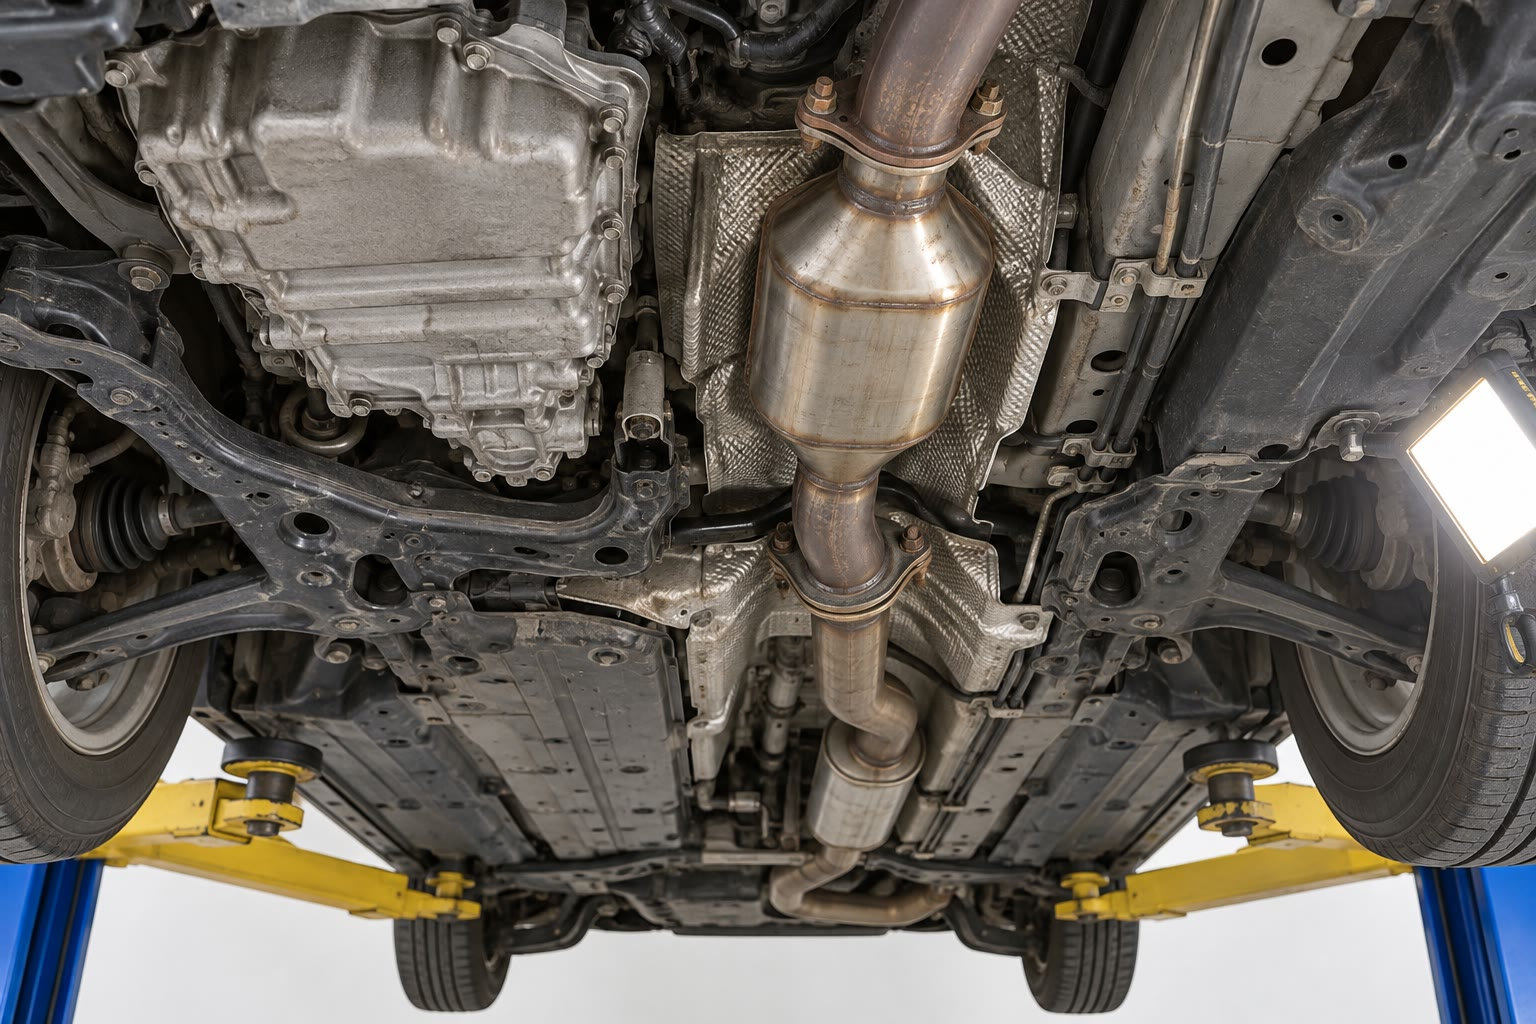
\includegraphics[width=0.5\linewidth]{images/book2/ai/b1-09-catalytic-converter.jpg}

{\small De onderkant van een auto: de bus in de uitlaatleiding is de
katalysator van de auto, een heterogene \omterm{def:b1:elementary-steps:catalyst}{katalysator} aan het
metaaloppervlak waarvan de uitlaatgassen reageren.}
\end{omfigure}

\begin{definition}[Kinetische en thermodynamische controle]\label{def:b1:elementary-steps:control}
Wanneer een beginstof via concurrerende paden twee producten kan geven,
staat de reactie onder \emph{kinetische controle}\index{kinetische controle}
als de verhoudingen van de producten bepaald worden door de
vormingssnelheden (het product met de laagste barrière overheerst), en
onder \emph{thermodynamische
controle}\index{thermodynamische controle} als de paden omkeerbaar zijn en
het systeem het evenwicht bereikt (het stabielste product overheerst).
\end{definition}

\begin{example}[Het product kiezen]\label{ex:b1:elementary-steps:control}
Een beginstof geeft B over een barrière van \qty{50}{kJ/mol} ($\Delta E =
\qty{-10}{kJ/mol}$) en C over een barrière van \qty{70}{kJ/mol}
($\Delta E =
\qty{-40}{kJ/mol}$). Bij \qty{300}{K} en korte tijden, met gelijke
\omterm{def:b1:rate-laws:activation-energy}{pre-exponentiële factoren}, wordt B $\exp(20000/(8.314 \times 300)) \approx
3000$ keer sneller gevormd dan C: \omterm{def:b1:elementary-steps:control}{kinetische controle} geeft B. Bij hoge
temperatuur en lange tijden keert B over zijn kleine terugbarrière terug,
C niet, en eindigt het systeem als C: \omterm{def:b1:elementary-steps:control}{thermodynamische controle}.
\end{example}

\begin{history}[Katalyse, 1835]
In 1835 bracht de Zweedse chemicus Jöns Jacob Berzelius een tiental
raadselachtige waarnemingen onder één woord samen --- zetmeel dat door
zuren in suiker wordt omgezet, waterstofperoxide dat door metalen
ontleed wordt, alcohol dat op platina oxideert --- en noemde hij de
verborgen kracht die daar werkte ``katalytisch''. Pas de kinetiek van het
einde van de eeuw, met Wilhelm Ostwald, definieerde een \omterm{def:b1:elementary-steps:catalyst}{katalysator} als
een deeltje dat de snelheid van een reactie verandert en niet haar
evenwicht.
\end{history}

\section{Oefeningen}

\begin{exercise}[$\star$]\label{exo:b1:elementary-steps:1}
Geef de \omterm{def:b1:elementary-steps:elementary-step}{moleculariteit} van elke stap en zeg welke stappen elementair
kunnen zijn:
(a) $\ce{N2O5 -> NO2 + NO3}$; (b) $\ce{NO + NO3 -> 2NO2}$;
(c) $\ce{2H2 + O2 -> 2H2O}$; (d) $\ce{O + O2 + N2 -> O3 + N2}$.
\end{exercise}

\begin{exercise}[$\star$]\label{exo:b1:elementary-steps:2}
Schrijf de \omterm{def:b1:rate-laws:order}{snelheidswet} op van de \omterm{def:b1:elementary-steps:elementary-step}{elementaire stappen} $\mathrm{A} + \mathrm{B} \to
\mathrm{C}$, $2\,\mathrm{A} \to \mathrm{B}$ en $\mathrm{A} \to \mathrm{B} +
\mathrm{C}$. Waarom kan de \omterm{def:b1:rate-laws:order}{snelheidswet} van een totale reactie niet uit
haar reactievergelijking worden afgeleid?
\end{exercise}

\begin{exercise}[$\star$]\label{exo:b1:elementary-steps:3}
Wijs op het \omterm{def:b1:elementary-steps:energy-profile}{energieprofiel} in twee stappen dat in dit hoofdstuk getekend
is (intermediair op 30, \omterm{def:b1:elementary-steps:energy-profile}{overgangstoestanden} op 70 en 55, producten op
$-40$, in \unit{kJ/mol} boven de beginstoffen) het intermediair, de
\omterm{def:b1:elementary-steps:energy-profile}{overgangstoestanden} en de \omterm{def:b1:elementary-steps:rds}{snelheidsbepalende stap} aan. Is de eerste stap
endotherm of exotherm?
\end{exercise}

\begin{exercise}[$\star$]\label{exo:b1:elementary-steps:4}
Een \omterm{def:b1:elementary-steps:catalyst}{katalysator} vermenigvuldigt de \omterm{def:b1:rate-laws:order}{snelheidsconstante} in de heenrichting
van een \omterm{def:b1:elementary-steps:elementary-step}{elementaire stap} met $10^4$. Met welke factor vermenigvuldigt hij
de \omterm{def:b1:rate-laws:order}{snelheidsconstante} in de terugrichting? De evenwichtsconstante? De
tijd die nodig is om het evenwicht te bereiken?
\end{exercise}

\begin{exercise}[$\star\star$]\label{exo:b1:elementary-steps:5}
Bereken voor $\mathrm{A} \to \mathrm{B} \to \mathrm{C}$ met $k_1 =
\qty{0.10}{s^{-1}}$ en $k_2 = \qty{0.30}{s^{-1}}$ het tijdstip $t_{\max}$
en de grootste concentratie van $\mathrm{B}$, in eenheden van $a_0$.
\end{exercise}

\begin{exercise}[$\star\star$]\label{exo:b1:elementary-steps:6}
Pas voor $\mathrm{A} \underset{k_{-1}}{\overset{k_1}{\rightleftharpoons}}
\mathrm{I} \xrightarrow{k_2} \mathrm{P}$, met alle stappen van orde 1, de
\omterm{def:b1:elementary-steps:qssa}{stationaire-toestandsbenadering} toe op $\mathrm{I}$ en toon aan dat $v =
\frac{k_1k_2}{k_{-1} + k_2}[\mathrm{A}]$. Bespreek de gevallen $k_2 \gg
k_{-1}$ en $k_2 \ll k_{-1}$.
\end{exercise}

\begin{exercise}[$\star\star$]\label{exo:b1:elementary-steps:7}
Jodide-ionen katalyseren de ontleding van waterstofperoxide:
\ce{H2O2 + I- -> H2O + IO-} (traag), daarna \ce{H2O2 + IO- -> H2O + O2 + I-}
(snel). Schrijf de totale reactievergelijking op, wijs de \omterm{def:b1:elementary-steps:catalyst}{katalysator} en
het intermediair aan, en geef de \omterm{def:b1:rate-laws:order}{snelheidswet}.
\end{exercise}

\begin{exercise}[$\star\star$]\label{exo:b1:elementary-steps:8}
Een stap vormt een carbokation uit een neutraal molecuul, een sterk
opwaarts proces. Leg met het postulaat van Hammond uit waarom een
substituent die het carbokation stabiliseert, ook de stap versnelt.
\end{exercise}

\begin{exercise}[$\star\star$]\label{exo:b1:elementary-steps:9}
Bereken in \cref{ex:b1:elementary-steps:control} de verhouding van de
\omterm{def:b1:rate-laws:order}{snelheidsconstanten} voor de vorming van B en C bij \qty{300}{K} en bij
\qty{600}{K}. Becommentarieer.
\end{exercise}

\begin{exercise}[$\star\star\star$]\label{exo:b1:elementary-steps:10}
Een gas $\mathrm{A}$ ontleedt nadat het geactiveerd is door een botsing
met een willekeurig molecuul $\mathrm{M}$:
$\mathrm{A} + \mathrm{M} \rightleftharpoons
\mathrm{A}^* + \mathrm{M}$ ($k_1$, $k_{-1}$), daarna $\mathrm{A}^* \to
\mathrm{P}$ ($k_2$). Bepaal met de \omterm{def:b1:elementary-steps:qssa}{stationaire-toestandsbenadering} voor
$\mathrm{A}^*$ de snelheid $v$, en toon aan dat de reactie bij hoge druk van orde 1
is en bij lage druk van orde 2.
\end{exercise}

\begin{exercise}[$\star\star\star$]\label{exo:b1:elementary-steps:11}
Bewijs de formule voor $[\mathrm{B}](t)$ van
\cref{thm:b1:elementary-steps:consecutive} en behandel het bijzondere
geval $k_1 = k_2 = k$, waarvoor $[\mathrm{B}] = a_0kt\,\eu^{-kt}$.
\end{exercise}

\begin{exercise}[$\star\star\star$]\label{exo:b1:elementary-steps:12}
De totale reactie $\mathrm{A} + 2\,\mathrm{B} \to \mathrm{P} +
\mathrm{C}$ heeft de experimentele \omterm{def:b1:rate-laws:order}{snelheidswet} $v =
k[\mathrm{A}][\mathrm{B}]^2/[\mathrm{C}]$. Stel een mechanisme met een snel
voorevenwicht voor dat haar verklaart.
\end{exercise}

\section{Probleem: waarom stikstofmonoxide in de kou sneller oxideert}

\begin{problem}[{Weekendprobleem --- de oxidatie van stikstofmonoxide van
de derde orde, een voorevenwicht via het dimeer \ce{N2O2}, de behandeling
met de stationaire toestand, en een negatieve schijnbare
\omterm{def:b1:rate-laws:activation-energy}{activeringsenergie}}]
\label{pb:b1:elementary-steps:1}
Voor \ce{2NO(g) + O2(g) -> 2NO2(g)} leveren metingen van de \omterm{def:b1:rate-laws:initial-rate}{beginsnelheid}
bij \qty{300}{K} (snelheden in \unit{mol.L^{-1}.s^{-1}}):
\begin{center}
\begin{tabular}{cccc}
\hline
experiment & $[\ce{NO}]_0$ (mol/L) & $[\ce{O2}]_0$ (mol/L) & $v_0$ \\
\hline
1 & \num{1.0e-3} & \num{1.0e-3} & \num{1.0e-5} \\
2 & \num{2.0e-3} & \num{1.0e-3} & \num{4.0e-5} \\
3 & \num{1.0e-3} & \num{2.0e-3} & \num{2.0e-5} \\
\hline
\end{tabular}
\end{center}
De \omterm{def:b1:rate-laws:order}{snelheidsconstante} die bij \qty{400}{K} gevonden wordt, is tien keer
kleiner dan bij \qty{300}{K}. Neem $R = \qty{8.314}{J/(mol.K)}$.
Het voorgestelde mechanisme is
\[
  \ce{2NO <=> N2O2} \ \ (k_1, k_{-1}, \text{snel}), \qquad
  \ce{N2O2 + O2 -> 2NO2} \ \ (k_2, \text{traag}).
\]

\medskip
\noindent\textbf{Deel I --- De waargenomen wet.}
\begin{enumerate}
  \item Bepaal de \omterm{def:b1:rate-laws:order}{partiële ordes} ten opzichte van \ce{NO} en \ce{O2}.
  \item Schrijf de \omterm{def:b1:rate-laws:order}{snelheidswet} op en bereken $k$ bij \qty{300}{K}, met
        zijn eenheid.
  \item Zou de reactie één enkele trimoleculaire stap kunnen zijn? Geef
        een argument.
  \item Bereken de schijnbare \omterm{def:b1:rate-laws:activation-energy}{activeringsenergie} uit de twee
        temperaturen.
  \item Waarom is een negatieve \omterm{def:b1:rate-laws:activation-energy}{activeringsenergie} onmogelijk voor een
        \omterm{def:b1:elementary-steps:elementary-step}{elementaire stap}?
  \item Schrijf de verdwijningssnelheden van \ce{NO} en \ce{O2} uit in
        termen van $v$.
\end{enumerate}

\medskip
\noindent\textbf{Deel II --- Het voorevenwicht.}
\begin{enumerate}[resume]
  \item Controleer dat de twee stappen samen de totale reactie geven.
        Benoem het intermediair.
  \item Geef de \omterm{def:b1:elementary-steps:elementary-step}{moleculariteit} van elke stap.
  \item Schrijf de snelheid van de trage stap op.
  \item Druk $[\ce{N2O2}]$ uit met de \omterm{def:b1:elementary-steps:pre-equilibrium}{voorevenwichtsbenadering}.
  \item Leid de \omterm{def:b1:rate-laws:order}{snelheidswet} af en vergelijk met het experiment.
  \item Druk de waargenomen constante uit met $k_1$, $k_{-1}$ en $k_2$.
\end{enumerate}

\medskip
\noindent\textbf{Deel III --- De stationaire toestand.}
\begin{enumerate}[resume]
  \item Schrijf $\dd[\ce{N2O2}]/\dd t$ op voor het volledige mechanisme.
  \item Pas de \omterm{def:b1:elementary-steps:qssa}{stationaire-toestandsbenadering} toe en druk $[\ce{N2O2}]$
        uit.
  \item Leid de \omterm{def:b1:rate-laws:order}{snelheidswet} $v = \dfrac{k_1k_2[\ce{NO}]^2[\ce{O2}]}{k_{-1} +
        k_2[\ce{O2}]}$ af.
  \item In welk grensgeval herleidt ze zich tot het resultaat van Deel II?
  \item Wat zouden de ordes worden in het tegengestelde grensgeval?
  \item Welk grensgeval ondersteunen de metingen van Deel I?
\end{enumerate}

\medskip
\noindent\textbf{Deel IV --- De schijnbare \omterm{def:b1:rate-laws:activation-energy}{activeringsenergie}.}
Elke stap volgt de \omterm{thm:b1:rate-laws:arrhenius}{wet van Arrhenius}, met activeringsenergieën $E_1 =
\qty{2}{kJ/mol}$, $E_{-1} = \qty{40}{kJ/mol}$ en $E_2 =
\qty{15}{kJ/mol}$.
\begin{enumerate}[resume]
  \item Druk $\ln k$ uit als functie van de logaritmen van $k_1$,
        $k_{-1}$ en $k_2$.
  \item Leid $E_a = E_1 - E_{-1} + E_2$ af.
  \item Interpreteer: waarom kan een combinatie van \omterm{def:b1:elementary-steps:elementary-step}{elementaire stappen}
        een negatieve schijnbare \omterm{def:b1:rate-laws:activation-energy}{activeringsenergie} hebben?
  \item Schets het \omterm{def:b1:elementary-steps:energy-profile}{energieprofiel}: waar ligt de tweede \omterm{def:b1:elementary-steps:energy-profile}{overgangstoestand}
        ten opzichte van de beginstoffen \ce{2NO + O2}?
  \item Met welke factor zou de snelheid met deze waarde veranderen tussen
        300 en \qty{400}{K}?
  \item Bereken de schijnbare \omterm{def:b1:rate-laws:activation-energy}{activeringsenergie} uit de waarden van de
        stappen, en vergelijk met Deel I.
\end{enumerate}
\end{problem}
